\documentclass[11pt]{article}
\usepackage[utf8]{inputenc}	% Para caracteres en español
\usepackage{amsmath,amsthm,amsfonts,amssymb,amscd}
\usepackage{multirow,booktabs}
\usepackage[table]{xcolor}
\usepackage{fullpage}
\usepackage{lastpage}
\usepackage{enumitem}
\usepackage{fancyhdr}
\usepackage{mathrsfs}
\usepackage{wrapfig}
\usepackage{setspace}
\usepackage{calc}
\usepackage{multicol}
\usepackage{cancel}
%\usepackage[retainorgcmds]{IEEEtrantools}
\usepackage[margin=3cm]{geometry}
\usepackage{amsmath}
\newlength{\tabcont}
\setlength{\parindent}{0.0in}
\setlength{\parskip}{0.05in}
\usepackage{empheq}
\usepackage{framed}
\usepackage[most]{tcolorbox}
\usepackage{xcolor}
\colorlet{shadecolor}{orange!15}
\parindent 0in
\parskip 12pt
\geometry{margin=1in, headsep=0.25in}
\theoremstyle{definition}
\newtheorem{defn}{Definition}
\newtheorem{reg}{Rule}
\newtheorem{exer}{Exercise}
\newtheorem{note}{Note}

%my additions
\usepackage{graphicx}
\usepackage{caption}
\usepackage{tikz}
\usetikzlibrary{bayesnet}
\usepackage{amsthm}
\usepackage{amsmath}
\usepackage{amsfonts}
\usepackage{amssymb}

% Bold shortcuts
\newcommand{\bb}[1]{\mathbf{#1}}
% - lowercase
\newcommand{\bbb}{\bb{b}}
\newcommand{\bx}{\bb{x}}
\newcommand{\bxi}{\bx^{(i)}}
\newcommand{\bxl}{\bx^{(l)}}
\newcommand{\bt}{\bb{t}}
\newcommand{\by}{\bb{y}}
\newcommand{\bv}{\bb{v}}
\newcommand{\bw}{\bb{w}}
\newcommand{\bc}{\bb{c}}
\newcommand{\bd}{\bb{d}}
\newcommand{\bg}{\bb{g}}
\newcommand{\bh}{\bb{h}}
\newcommand{\br}{\bb{r}}
\newcommand{\bu}{\bb{u}}
\newcommand{\byl}{\by^{(l)}}
\newcommand{\bz}{\bb{z}}
\newcommand{\bzi}{\bz^{(i)}}
\newcommand{\bzl}{\bz^{(l)}}
\newcommand{\bzil}{\bz^{(i,l)}}
\newcommand{\bpa}{\bb{pa}}

\newcommand{\bT}{\boldsymbol{\theta}}
\newcommand{\bTl}{\boldsymbol{\theta}^{(l)}}
\newcommand{\balpha}{\boldsymbol{\alpha}}
\newcommand{\bphi}{\boldsymbol{\phi}}
\newcommand{\beps}{\boldsymbol{\epsilon}}
\newcommand{\bepsl}{\beps^{(l)}}
\newcommand{\bepsil}{\beps^{(i,l)}}
\newcommand{\bzeta}{\boldsymbol{\zeta}}
\newcommand{\bzetal}{\zeta^{(l)}}
\newcommand{\bsigma}{\boldsymbol{\sigma}}
\newcommand{\bmu}{\boldsymbol{\mu}}
\newcommand{\bzero}{\bb{0}}

% - uppercase
\newcommand{\bL}{\bb{L}}
\newcommand{\bV}{\bb{V}}
\newcommand{\bW}{\bb{W}}
\newcommand{\bI}{\bb{I}}
\newcommand{\bR}{\bb{R}}
\newcommand{\bX}{\bb{X}}
\newcommand{\bO}{\bb{O}}

\newcommand{\btPa}{\widetilde{\bb{Pa}}}
\newcommand{\btpa}{\widetilde{\bb{pa}}}

% Tilde
\newcommand{\tz}{\widetilde{z}}
\newcommand{\tZ}{\widetilde{Z}}
\newcommand{\tf}{\widetilde{f}}
\newcommand{\btZ}{\widetilde{\bb{Z}}}
\newcommand{\btz}{\widetilde{\bz}}
\newcommand{\btT}{\widetilde{\bT}}
\newcommand{\tPa}{\widetilde{Pa}}

\newcommand{\pT}{p_{\bT}}
\newcommand{\pTl}{p_{\bT^{(l)}}}
\newcommand{\pA}{p_{\balpha}}
\newcommand{\qT}{q_{\bT}}
\newcommand{\qPhi}{q_{\bphi}}
\newcommand{\fT}{f_{\bT}}
\newcommand{\fPhi}{f_{\bphi}}
\newcommand{\fTPhi}{f_{\bT,\bphi}}
\newcommand{\gT}{g_{\bT}}
\newcommand{\gPhi}{g_{\bphi}}
\newcommand{\hPhi}{h_{\bphi}}

\newcommand{\Exp}[2]{\mathbb{E}_{#1}\left[#2\right]}
\newcommand{\Ed}{\mathbb{E}_\bd}
\newcommand{\eqnr}{\addtocounter{equation}{1}\tag{\theequation}}

\DeclareMathOperator*{\argmax}{argmax}

% Create 'example' environment
\theoremstyle{definition}
\newtheorem{exmp}{Example}[section]

% Variational bound
\newcommand{\LB}[2]{\mathcal{L}^{#1}(\bT,\bphi; #2)}
\newcommand{\LBT}[2]{\widetilde{\mathcal{L}}^{#1}(\bT,\bphi; #2)}
 %to use the commands by kingma and welling
%for figure referencing in-text
\usepackage[hidelinks]{hyperref}
\usepackage{cleveref}
%for biliography
\usepackage[backend=bibtex,style=authoryear-comp,natbib=true]{biblatex} % Use the bibtex backend with the authoryear citation style (which resembles APA)
\addbibresource{vae.bib} % The filename of the bibliography

%for drawing boxes around text
\usepackage[linewidth=1pt]{mdframed}

%for under- and overbrace
\usepackage{mathtools}


\begin{document}

\thispagestyle{empty}

%------------------------------
%	HEADLINE
%------------------------------
\begin{center}
{\LARGE \bf Concept Notes: The Variational Auto-Encoder}\\
{\large Luis Oala}\\
\today
\end{center}

%------------------------------
%	DOCUMENT
%------------------------------
\section{Setting: The Situation}

\begin{figure}[h]
	\begin{center}
		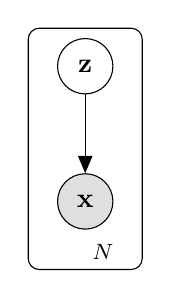
\begin{tikzpicture}[scale=1, transform shape]
		\node[obs] (x1) {$\mathbf{x}$};
		\node[latent, above=of x1] (z1) {$\mathbf{z}$};
		\edge {z1} {x1};
		\plate [xscale=1.5] {} {(x1)(z1)} {$N$} ;
		\end{tikzpicture}
	\end{center}
	\caption{
		We can observe, i.e. actually see, $N$ samples of the random variable $\bx$. We assume that $\bx$ depends on another variable $\bz$, which is latent , i.e. we cannot observe it. Graph adapted from \citep{kingma_auto-encoding_2013}.
	}
	\label{fig:situation}
\end{figure}

Imagine a situation as depicted in \autoref{fig:situation}. Our situation includes the following ingredients, assumptions and constraints:
\begin{itemize}
	\item A size $N$ observed sample $\mathbf{X}$ of random variable $\mathbf{x}$. We \underline{assume} that $\bx$ follows the \textit{likelihood} $p_{\bT^*}(\bx|\bz)$.
	\item A latent variable $\bz$ which we \underline{assume} to follow the \textit{prior} $p_{\bT^*}(\bz)$. It is called latent because we cannot see any of the $\bz$ values.
	\item We \underline{assume} that $p_{\bT^*}(\bz)$ and $p_{\bT^*}(\bx|bz)$ belong to the parametric family of distributions $p_{\bT}(\bz)$ and $p_{\bT}(\bx|\bz)$.
	\item We do not know anything about $\bT^*$ or $\bz$.
\end{itemize}

\begin{mdframed}
	{\Large \bf Basic probability rules reference}
		\begin{equation}
			p(\bx, \bz) = p(\bx|\bz)p(\bz)
			\label{eq:joint}
		\end{equation}
		
		\begin{equation}
			p(\bx) = \int p(\bx, \bz) d\bz
			\label{eq:marg}
		\end{equation}
		
		\begin{equation}
		\text{Bayes' Theorem:} \overbrace{p(\bz|\bx)}^{\textit{posterior}}=\frac{\overbrace{p(\bx|\bz)}^{\textit{likelihood}}\overbrace{p(\bz)}^{\textit{prior}}}{\underbrace{p(\bx)}_{\textit{evidence}}}
		\label{eq:bayes}
		\end{equation}
\end{mdframed}


\section{The goal}
We want to learn what sensible values for our unknown, latent variable $\bz$ would be given the information we have available. Bayes' formula gives us a straightforward way to do so. We are interested in the \textit{posterior} $\pT(\bz|\bx)$.

\section{The approach}
\subsection{Getting started}
For a given $\bT$ we have all the ingredients to calculate the \textit{posterior} $\pT(\bz|\bx)$ using Bayes' formula (\autoref{eq:bayes}):
\begin{equation}
	\pT(\bz|\bx)=\frac{\pT(\bx|\bz)\pT(\bz)}{\pT(\bx)}
	\label{eq:bayes-post-theta}
\end{equation}
Remember that per our initial assumption we have access to $p_{\bT}(\bz)$ and $p_{\bT}(\bx|\bz)$ for some $\bT$. We just do not know the true $\bT^*$. Via \autoref{eq:marg} we have, in theory, access to the \textit{evidence} $\pT(\bx)$ as well.
\par
So we can calculate, again \underline{in theory}, the \textit{posterior} $\pT(\bz|\bx)$ ...

\subsection{Problem 1: Intractable  $\pT(\bx)$}
... but the integration over all possible values of $\bz$ in \autoref{eq:marg} is computationally not feasible (TODO: why actually not?). That means we cannot calculate $\pT(\bz|\bx)$ simply using Bayes after all.

\subsection{Idea for Solution to Problem 1: What about using $D_{\text{KL}}$?}
Okay, so we cannot simply calculate $\pT(\bz|\bx)$ with the information available at our disposal. What about this idea: We try to approximate $\pT(\bz|\bx)$ using a parametric distribution $\qPhi(\bz|\bx)$ by doing
\begin{equation}
	\underset{\bphi}{\mathrm{argmin}} D_{\text{KL}}(\qPhi(\bz|\bx)||\pT(\bz|\bx))
	\label{eq:min-dkl}
\end{equation}
The $\qPhi(\bz|\bx)$ with the problematic $\pT(\bx)$ is still part \autoref{eq:min-dkl}, but maybe with some wishful thinking and function magic the $D_{KL}$ is somehow getting rid of it? Let us see:
\begin{equation}
	D_{\text{KL}}(\qPhi(\bz|\bx)||\pT(\bz|\bx)) = \mathbb{E}_{\qPhi(\bz|\bx)}[\log \qPhi(\bz|\bx)] - \mathbb{E}_{\qPhi(\bz|\bx)}[\log \pT(\bx,\bz)] + \log\pT(\bx)
	\label{eq:dkl-full1}
\end{equation}
TODO: include the derivation for \autoref{eq:dkl-full1} from page 12 of your notes. This also covers the ELBO derivation part  \par
Unfortunately, the answer is no. $\log\pT(\bx)$ is still part of the expression. No magic, we are back to square one.

\subsection{Actual Solution to Problem 1: Use your ELBO}
But our efforts in the previous step, using the $D_{\text{KL}}$, were not in vain. Upon closer examination of \autoref{eq:dkl-full1} the first two terms turn out to be part of a familiar expression: the evidence lower bound (ELBO). Viewed as a function of $\bphi$ and $\bT$ the ELBO is defined as:
\begin{equation}
	\mathbf{ELBO}(\bphi, \bT) = \mathbb{E}_{\qPhi(\bz|\bx)}[\log \pT(\bx,\bz)] - \mathbb{E}_{\qPhi(\bz|\bx)}[\log \qPhi(\bz|\bx)]
	\label{eq:elbo}
\end{equation}
Note that the ELBO is a function of $\pT(\bx,\bz)$ and $\qPhi(\bz|\bx)$, all things we have access to and can compute with. That sounds promising! We can reformulate \autoref{eq:dkl-full1} by inserting the $\mathbf{ELBO}(\bphi, \bT)$ as such:
\begin{equation}
	D_{\text{KL}}(\qPhi(\bz|\bx)||\pT(\bz|\bx)) = \log\pT(\bx) - \mathbf{ELBO}(\bphi, \bT)
	\label{eq:dkl-with-elbo}
\end{equation}
In \autoref{eq:dkl-with-elbo} it also becomes apparant why the ELBO is called ELBO. When rearranging \autoref{eq:dkl-with-elbo} we get
\begin{equation}
	\log\pT(\bx) = \underbrace{D_{\text{KL}}(\qPhi(\bz|\bx)||\pT(\bz|\bx))}_{\geq 0} + \mathbf{ELBO}(\bphi, \bT)
	\label{eq:elbo-as-lower-bound1}
\end{equation}
\begin{equation}
\log\pT(\bx) \geq \mathbf{ELBO}(\bphi, \bT)
\label{eq:elbo-as-lower-bound2}
\end{equation}
Thus we can see that the ELBO indeed is a lower bound to the likelihood of the \textit{evidence}. We can also rewrite \autoref{eq:elbo} as: (TODO: include detailed derivation and clean point about this single datapoint vs. all decomposition of the objective)
\begin{equation}
	\mathbf{ELBO}(\bphi, \bT) = \mathbb{E}_{\qPhi(\bz|\bx)}[\log \pT(\bx|\bz)] - D_{\text{KL}}(\qPhi(\bz|\bx)|p_{\bT}(\bz))
	\label{eq:elbo-final}
\end{equation}
\par 
Let us take a step back and recap what we have seen so far. Our initial goal was to learn about plausible values for $\bz$, a latent variable that we cannot observe. Bayes' Theorem gives us a straightforward way to reason about about $\bz$ by using the information we have on $p_{\bT}(\bz)$ and $p_{\bT}(\bx|\bz)$. Unfortunately we run into problems approximating the \textit{posterior} $\pT(\bz|\bx)$ because the computation of the \textit{evidence} $\pT(\bx)$ is intractable. We thought about using a parametric model $\qPhi((\bz|\bx))$ to minimize the $D_{\text{KL}}$ to the \textit{posterior} $\pT(\bz|\bx)$, but saw that the intractable $\pT(\bx)$ is still in the expression. So far so good. 
\par 
Our initial motivation for using the $D_\text{KL}$ was to have an objective that we can minimize to learn about the \textit{posterior} $\pT(\bz|\bx)$. If we now stare at \autoref{eq:dkl-with-elbo} for a while we can realize the following. At the optimal $\bphi^*$ we have that $	D_{\text{KL}}(q_{\bphi^*}(\bz|\bx)||\pT(\bz|\bx)) = 0$. Additionally we know that $\log\pT(\bx) \geq \mathbf{ELBO}(\bphi, \bT)$ from \autoref{eq:elbo-as-lower-bound2}. Since only the ELBO is a function of $\bphi$ (see RHS of \autoref{eq:dkl-with-elbo}) our objective of minimizing the $D_{\text{KL}}$ (LHS of \autoref{eq:dkl-with-elbo}) is equivalent to maximizing the ELBO w.r.t. $\bphi$. And this is what we will do for \textit{variational inference}. Finally we have a tractable approach to approximate the \textit{posterior} $\pT(\bz|\bx)$ and learn about plausible values for $\bz$ given our available data $\bx$: we maximize the ELBO!

\subsection{While we are at it: Let us learn about $\pT(\bx)$, too! }
We learned that \textit{evidence}  $\pT(\bx)$ is major culprit for all our problems. It is the reason why we have to take the tiresome detour via the ELBO to find a tractable optimization problem that satisfies our goal of learning about $\bz$. Along the way we learned that ELBO is called ELBO because it is a lower bound to the likelihood of the \textit{evidence}. We said previously that we will maximize the ELBO w.r.t. the variational parameters $\bphi$ because this is equivalent to minimizing the $D_{\text{KL}}$. But as we know from \autoref{eq:elbo-as-lower-bound2} (and from its name) the ELBO lower bounds the likelihood of the \textit{evidence}  $\pT(\bx)$. Thus if we want to learn and model the data $\bx$ as well we can do so by maximizing the ELBO w.r.t. $\bT$, too! And this is what happens in Variational Auto-Encoders: next to the \textit{variational inference} on the parameters $\bphi$ underlying variable $\bz$ we also perform \textit{variational expectation maximization} on the parameters $\bT$ underlying variable $\bx$.

\subsection{Keeping the concepts apart, clear and concise}
Just to reiterate and manifest the terminology (to me at least this is very important to keep the concepts ordered in my head).

\begin{itemize}
	\item \textit{Variational inference}
	\begin{itemize}
		\item Keep $\bT$ fixed and do $\underset{\bphi}{\mathrm{argmax}} \ \mathbf{ELBO} (\bphi, \bT)$
		\item Allows us to learn about the latent variable $\bz$ via the approximated, parametric posterior $\qPhi(\bz|\bx)$
	\end{itemize}
	\item \textit{Variational EM (expectation maximization)}
	\begin{itemize}
		\item Keep $\bphi$ fixed and do $\underset{\bT}{\mathrm{argmax}} \ \mathbf{ELBO} (\bphi, \bT)$
		\item Allows us to learn about the observable variable $\bx$ via the available, parametric densities $p_{\bT}(\bz)$ and $p_{\bT}(\bx|\bz)$.
	\end{itemize}
\end{itemize}

\subsection{Putting it all together}
So we learned that in Variational Auto-Encoders we do not just perform \textit{variational inference} on the parameters of the latent variable but also learn a generative model of the observable data at the same time. Let us put all these parts together into a graphical representation for better overview:

\begin{figure}[t]
	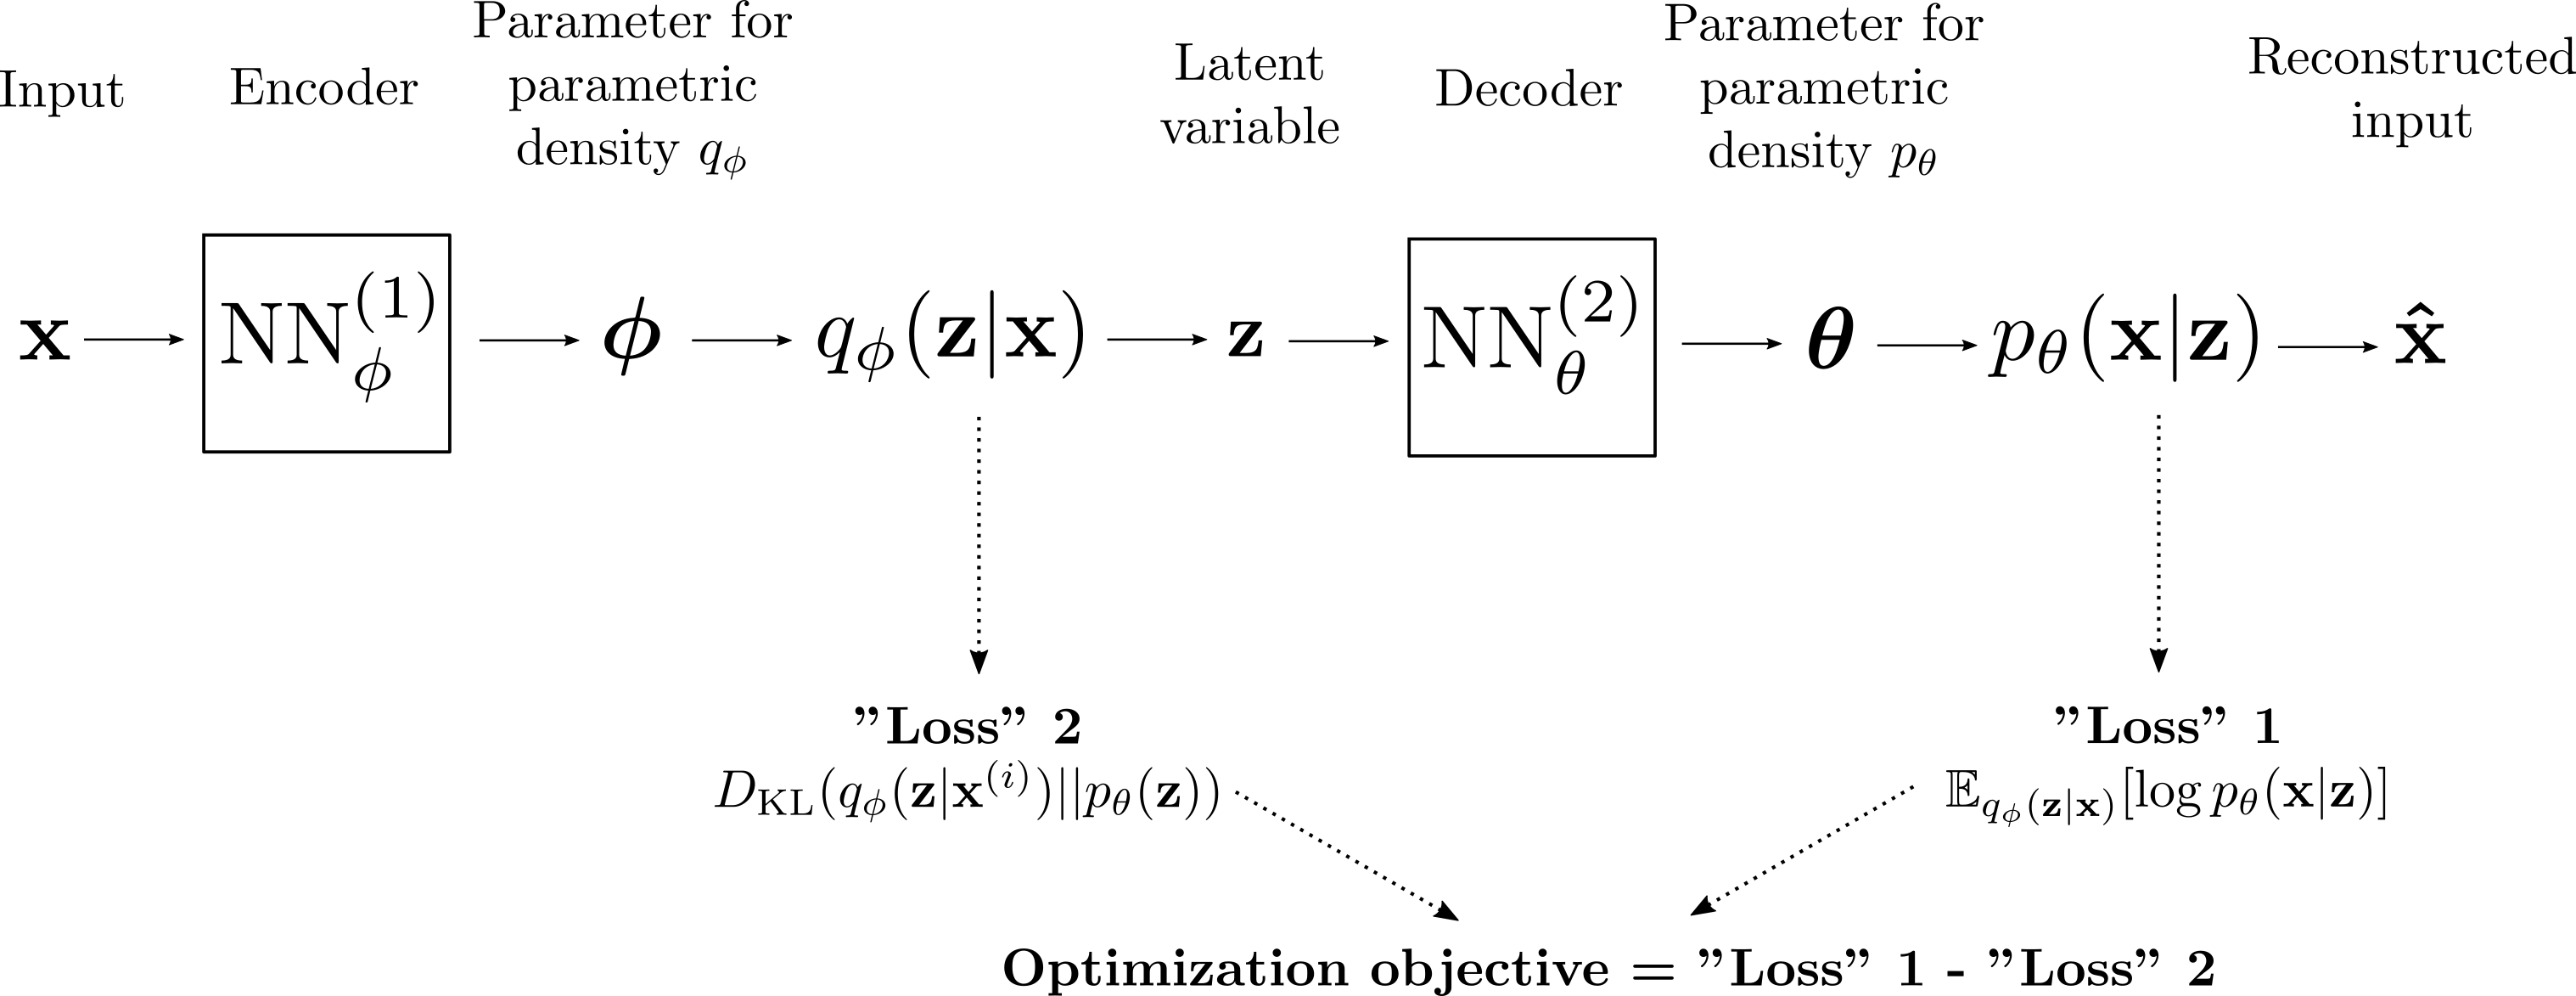
\includegraphics[width=\linewidth]{figures/vae-graph.png}
	\label{fig:vae-graph}
\end{figure}
\par 
Finally, a few short notes on how we can, in practice, evaluate the individual terms in the ELBO objective ( \autoref{eq:elbo-final}):
\begin{itemize}
	\item $\mathbb{E}_{\qPhi(\bz|\bx)}[\log \pT(\bx|\bz)]$
	\begin{itemize}
		\item Sampling based (sample several $\bz$ for a particular $\bx^{(i)}$ and take empirical agerage)
	\end{itemize}
	\item $D_{\text{KL}}(\qPhi(\bz|\bx)|p_{\bT}(\bz))$
	\begin{itemize}
		\item Sampling based (sample several $\bz$ for a particular $\bx^{(i)}$ and take empirical agerage)
		\item Analytically (e.g. this is possible if $\qPhi$ and $\pT$ are both Gaussian\footnote{See the appendix for such an example})
	\end{itemize}
\end{itemize}
For practical recommendations regarding the sampling procedure please check the original paper by \citep{kingma_auto-encoding_2013}. They have a number of tips.
\end{document}
